\documentclass[12pt]{beamer}
\usetheme{Madrid}
\usepackage[utf8]{inputenc}
\usepackage{amsmath}
\usepackage{amsfonts}
\usepackage{amssymb}
\usepackage{graphicx}
\usepackage{subfig}
\usepackage{float}

\title[LaBRi]{Deep learning meets the old times}
\author[Tu VU]{} % Your name
\institute[LaBRi]{}
\date{\today}
%\setbeamercovered{transparent} 
\setbeamertemplate{caption}[numbered]
%\logo{} 
%\institute{} 
%\date{} 
%\subject{} 
\AtBeginSubsection[]
{
  \begin{frame}<beamer>{Outline}
    \tableofcontents[currentsection,currentsubsection]
  \end{frame}
}
\AtBeginSection[]
{
  \begin{frame}<beamer>{Outline}
    \tableofcontents[currentsection]
  \end{frame}
}
\begin{document}

\begin{frame}
\titlepage
\end{frame}

\section{Extracting Fragment’s Physical Attributes}
\subsection{Preprocessing}
\begin{frame}{Computing image dpi}
\begin{itemize}
\item A reference image of the ruler was photographed independently
\item The identification is done by employing a randomized algorithm: RANSAC
(Fischler and Bolles, 1981), combines with scale-invariant feature transform (SIFT) keypoint matching (Lowe, 2004)
\item For the latter task, a classical method such as the binarization method of (Sauvola and Pietikäinen, 2000) that also contains a method for identifying textual regions could be used
\end{itemize}
\end{frame}

\begin{frame}{Separating foreground from background}
The goal of this step is to detect the image of the fragment itself, isolating it from the accompanying background
\begin{itemize}
\item an automatic classifier was first applied to identify foreground pixels (in contrast to background ones Figure \ref{fig:contrast}) based on RGB color values (or HSV values)
\item create a region-based segmentation of the fragment(s), the connected components of the detected foreground pixels were marked
\item the convex hull of each component calculated (connected component = a contiguous region of foreground pixels; convex hull = the smallest possible encompassing polygon with angles opening inward)
\end{itemize}
\end{frame}

\begin{frame}
\begin{figure}[H]
	\subfloat[\label{fig:contrasta}]{
       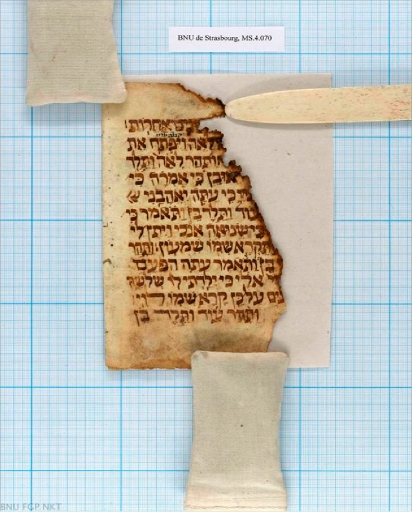
\includegraphics[width=0.35\textwidth]{images/1a.JPG}
     }
     \hfill
     \subfloat[\label{fig:contrastb}]{
       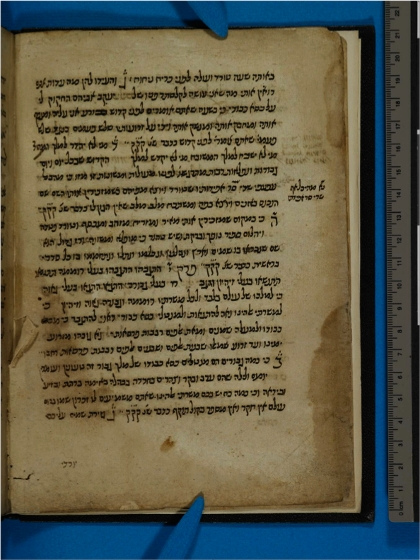
\includegraphics[width=0.35\textwidth]{images/1b.JPG}
     }\\
     \caption{(a) Fragment from the Strasbourg collection with label, clip and weight bags vs. (b) one from the British Library using a contrasting color}\label{fig:contrast}
\end{figure}
\end{frame}

\begin{frame}{Detecting and removing irrelevant components}
\begin{itemize}
\item In some collections, The system detected the binders (Figure \ref{fig:binder}) by the combination of their color and shape, and removed them from the image
\item In other collections, images included a label (Figure \ref{fig:contrasta})
with the fragment’s shelfmark. These labels were also detected by the
system and ignored
\end{itemize}
\end{frame}

\begin{frame}
\begin{figure}
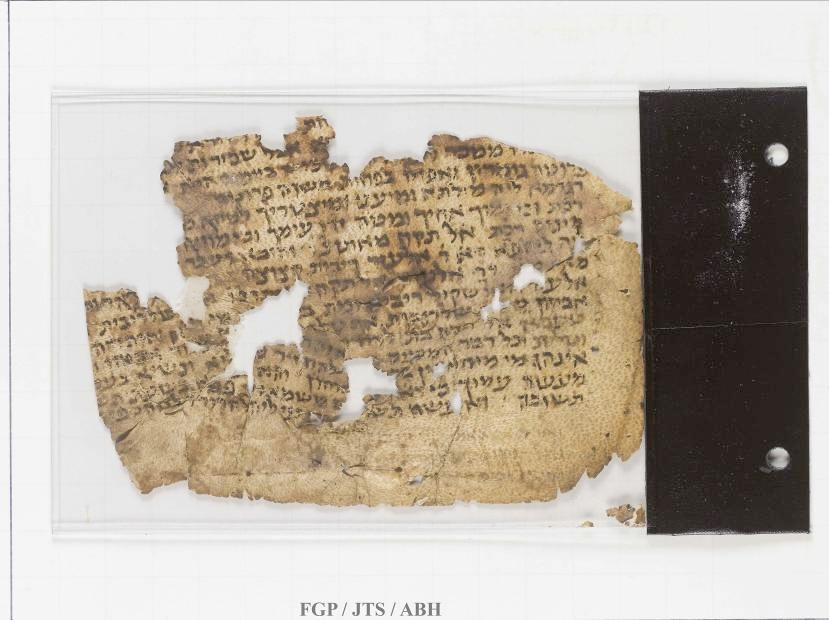
\includegraphics[width=0.8\textwidth]{images/2.JPG}
\caption{Fragment from the JTS collection with a black binder.}\label{fig:binder}
\end{figure}
\end{frame}

\begin{frame}{Separating multi-fragment images into components}
\begin{itemize}
\item In many cases, more than one fragment was captured in a single image (Figure \ref{fig:multifragment})
\item Each fragment (a “component” of the image) was identified and given a unique identifier (serial number) and handled independently.
\item However, there was a need to relate the components in the recto image of a fragment to the ones in its verso image (so as to have the same identifiers for both images)
\item This was done automatically by mirroring one image and matching the components in both images by size and shape
\end{itemize}
\end{frame}

\begin{frame}
\begin{figure}
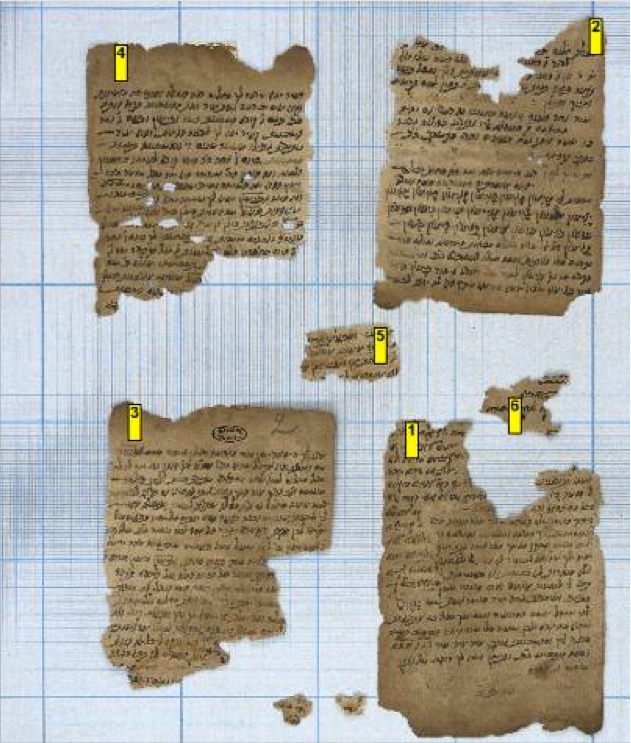
\includegraphics[height=0.6\textwidth]{images/3.JPG}
\caption{Multiple fragments in one image.}\label{fig:multifragment}
\end{figure}
\end{frame}

\begin{frame}{Binarization}
\begin{itemize}
\item The regions detected are then binarized, that is, every ink pixel is assigned a value of 1(representing black), and all other pixels are assigned a value of 0 (for white)
\item This is done using the auto-binarization tool of the ImageXpress 9.0 package by Accusoft Pegasus
\item ??
\end{itemize}
\end{frame}

\begin{frame}{Auto-alignment}
\begin{itemize}
\item Most cases fragments were imaged placed upright, in many other cases the fragment was tilted.
\item The need for alignment is two-fold:
\begin{itemize}
\item first, to enable the correct measurement of the fragment’s various attributes
\item second, to enable proper application of the handwriting-matching algorithm
\end{itemize}
\item Alignment is achieved by rotating the image until the lines of text are horizontal, using a simple method akin to those in (Baird, 1992, Srihari and Govindaraju, 1989)
\end{itemize}
\end{frame}
\end{document}ocument}